  \subsection{Enroll to a scheduled run}
After visualizing the list of scheduled runs, the User can choose one of them and, if there are available entries, can enroll to the chosen run. 

\begin{table}[H]
	\centering
    
    \begin{tabular}{|p{3.5cm}|p{10.3cm}|}
    
    \hline
    \textbf{\large{Actors}}  			& \tabitem User\\
    				 					
    \hline
    \textbf{\large{Goals}} 				& \ref{goal:run2}\\
    
    \hline
    \textbf{\large{Enter Condition}}	& The \emph{User} has already visualize the list of scheduled runs.\\
    
    \hline
    \textbf{\large{Events Flow}}		& \begin{enumerate}[leftmargin=0.5cm]
                                          	\item The \emph{User} chooses a run from the list of scheduled runs. 
                                          	 \item The System shows the details relative to the chosen run.
                                            \item The \emph{User} enrolls to the chosen run selecting the "Enroll" button.
                                            \item If there are available entries, the System adds the \emph{User} to the list of partecipants of the run.
                                             \item The System sends an email with all the informations about the run, the ticket's code and the bib number to the User's email address.
                                              \item The System notifies the \emph{User} through email updates in case of scheduling changes before the day of the run.
                                             \end{enumerate}
    										\\
    \hline
    \textbf{\large{Exit Conditions}}    & The User is enrolled to the run and added to the list of partecipants of the chosen run.  \\
    
    \hline
    \textbf{\large{Exceptions}} 		& \begin{enumerate}[leftmargin=0.5cm]
                                          	\item The \emph{User} tried to enroll to a run that has no more available entries.
                                          \end{enumerate}
    										If this problem occurs, the system shows an error message to the user, which is invited to choose another run.\\
    
    \hline
    
    \end{tabular}
	
\end{table}

\begin{figure}[H]
    \centering
    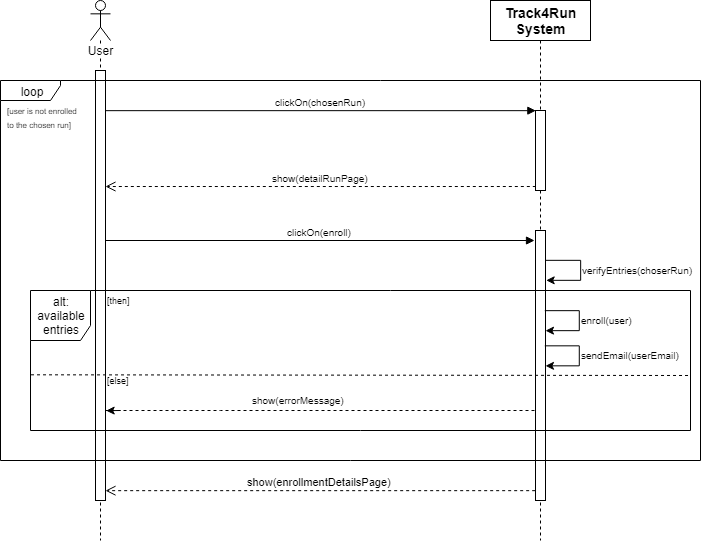
\includegraphics[scale=0.4]{Pictures/enrollSeqDiag.png}
    \caption{Sequence diagram for the enrollment of a user to a scheduled run}
\end{figure}
